\documentclass[12pt]{article}
\usepackage[utf8]{inputenc}
\usepackage{amsmath}
\usepackage[margin=1in]{geometry}
\usepackage{tikz}
\usepackage{blindtext}
\usepackage{graphicx}
\usepackage{float}
\usepackage[hidelinks]{hyperref}

\title{Week 9 Notes}
\author{Dylan Ang}
\date{May 2021}

\begin{document}

\maketitle

\tableofcontents

% ========== ========== ========== ==========

\section{Biogeochemistry}

\subsection{Carbon}

\subsubsection{The Global Carbon Cycle}

% \begin{figure}[H]
%     \centering
%     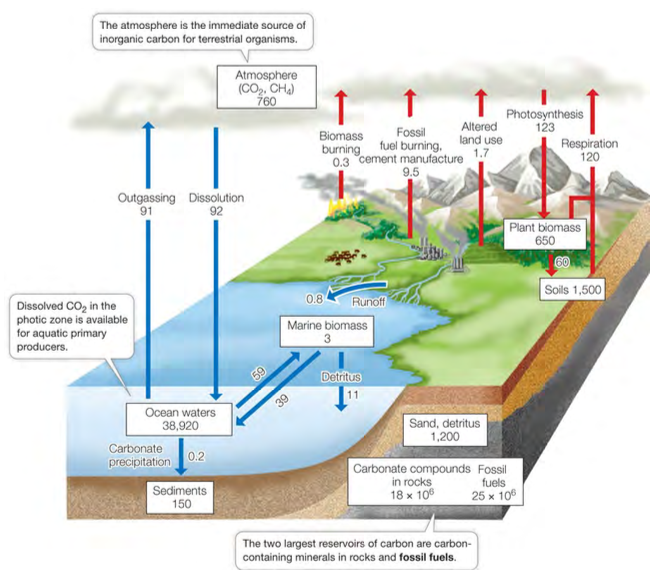
\includegraphics[width=5in]{global-carbon-cycle.png}
%     \caption{The Global Carbon Cycle}
%     \label{global-carbon-cycle}
% \end{figure}

\paragraph{In Figure \ref{global-carbon}}
\begin{itemize}
    \item Boxes represent carbon pools
          \begin{itemize}
              \item A carbon pool is a specific area in the ecosystem where carbon can exist.
              \item Pools with a higher number store more carbon mass, the largest being Rock Components and Fossil Fuels. However, there are no arrows coming off of these, so the largest pool that is active is Ocean Waters.
          \end{itemize}
    \item Arrows represent Fluxes.
          \begin{itemize}
              \item Fluxes represent processes that cause movement of carbon from one pool to another.
              \item Fluxes with a higher number transfer more carbon mass. The largest being photosynthesis.
          \end{itemize}
\end{itemize}

\begin{figure}[H]
    \centering
    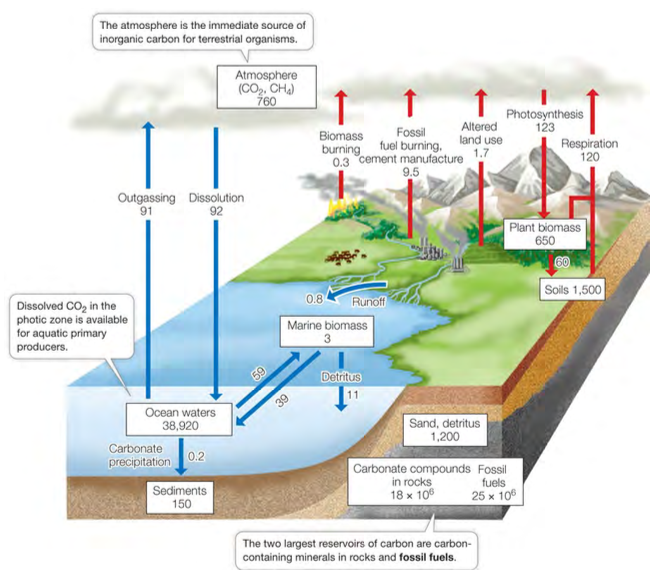
\includegraphics[width=5in]{global-carbon-cycle.png}
    \caption{The Global Carbon Cycle}
    \label{global-carbon}
\end{figure}

\subsubsection[Atmospheric Carbon Dioxide Levels]{Atmospheric $CO_2$ Levels}

\begin{figure}[tph]
    \centering
    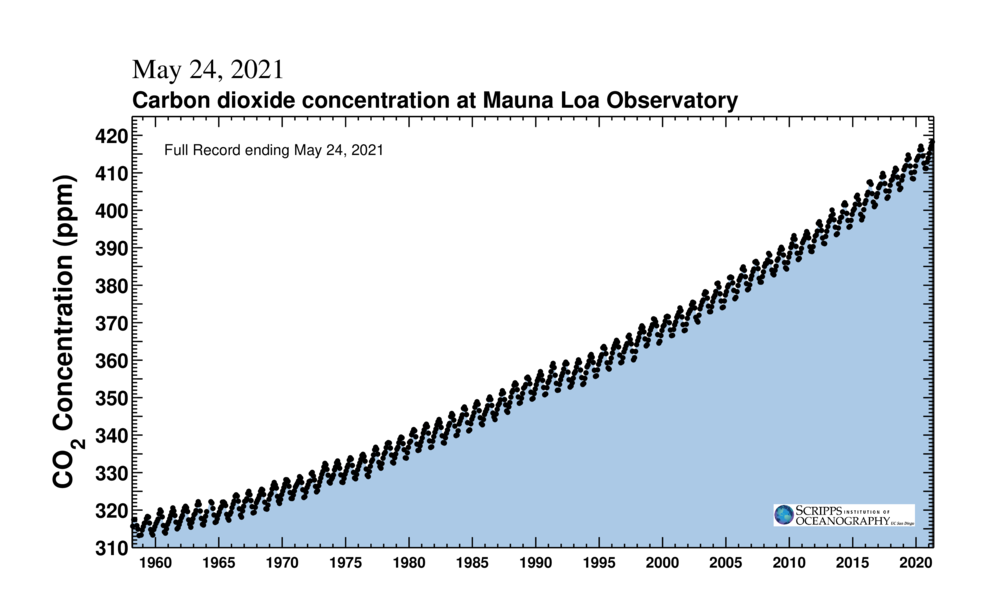
\includegraphics[width=5in]{keeling-curve.png}
    \caption{The Keeling Curve}
    \label{keeling-curve}
\end{figure}

\paragraph{Questions: in Figure \ref{keeling-curve}}
\begin{itemize}
    \item What process drives the overall increase in $CO_2$ levels?
          \begin{itemize}
              \item Anthropogenic greenhouse emissions: fossil fuels.
          \end{itemize}
    \item What process drives the annual oscillation in $CO_2$ levels?
          \begin{itemize}
              \item Global photosynthesis absorbs more $CO_2$ than Respiration creates when plants are growing, i.e., May to September.
              \item Global photosynthesis absorbs less $CO_2$ than Respiration creates when plants are not growing.
          \end{itemize}
    \item Highly seasonal, highly productive ecosystems like boreal forests will experience the most oscillation of $CO_2$ levels, because the carbon they absorb in Spring and Summer is not offset enough by the Southern hemisphere's Fall and Winter.
          \begin{itemize}
              \item Global $CO_2$ level oscillations are mainly driven by the boreal forest.
              \item Locations such as Mauna Loa or the South Pole will also see oscillations, although these are actually residual effects of the boreal forest.
              \item Locations that are not highly seasonal or highly productive will not be able to contribute to global $CO_2$ level oscillations.
          \end{itemize}
\end{itemize}

\paragraph{Ocean Acidification Example}
\begin{itemize}
    \item Higher Acidity (lower pH) and warming of ocean bleaches coral.
    \item Coral have an mutualistic relationship with zooxanthellae.
          \begin{itemize}
              \item Coral get sugar from photosynthesis of zooxanthellae.
              \item Zooxanthellae gets place to live, and nutrients from coral.
              \item Also obligate relationship for coral. Coral can not survive without the relationship.
          \end{itemize}
    \item Higher acidity or warming of the ocean acts as a stressor, killing zooxanthellae.
    \item Without the presence of zooxanthellae, the coral will lose its color (Coral Bleaching) and eventually die if prolonged. If conditions improve after bleaching but before death, the coral can recover by recruiting new zooxanthellae.
\end{itemize}

\subsection{Water and Nitrogen}

\subsubsection{The Global Hydrological Cycle}

\begin{figure}[tph]
    \centering
    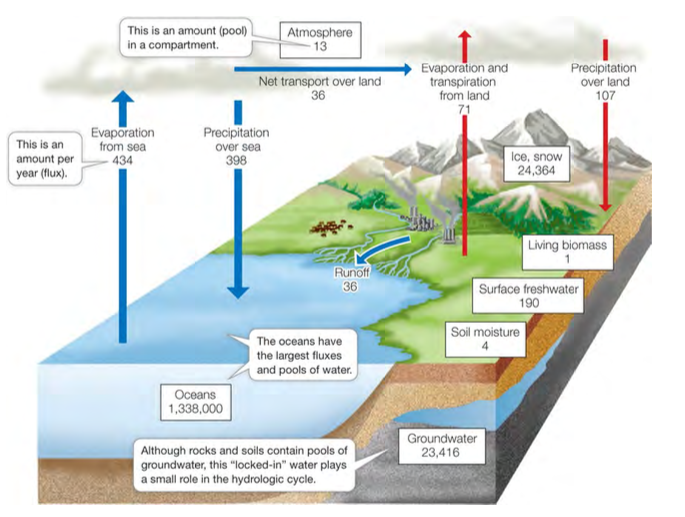
\includegraphics[width=5in]{global-hydrological-cycle.png}
    \caption{The Global Hydrological Cycle}
    \label{global-hydrological}
\end{figure}

\paragraph{In Figure \ref{global-hydrological}: The Global Hydrological Cycle}
\begin{itemize}
    \item Fluxes are processes by which water moves from one pool to another.
          \begin{itemize}
              \item Evaporation
              \item Transpiration
              \item Rain
          \end{itemize}
    \item Pools are locations that store water.
          \begin{itemize}
              \item Oceans
              \item Lakes
              \item Groundwater
          \end{itemize}
    \item Largest
          \begin{itemize}
              \item Flux: Evaporation from oceans
              \item Pool: Oceans
          \end{itemize}
    \item Anthropogenic Fluxes
          \begin{itemize}
              \item Groundwater does not naturally connect to the rest of the hydrological cycle.
              \item Humans can, through irrigation and aquifers, access groundwater and thus connect it to the cycle.
          \end{itemize}
\end{itemize}

\begin{figure}[tph]
    \centering
    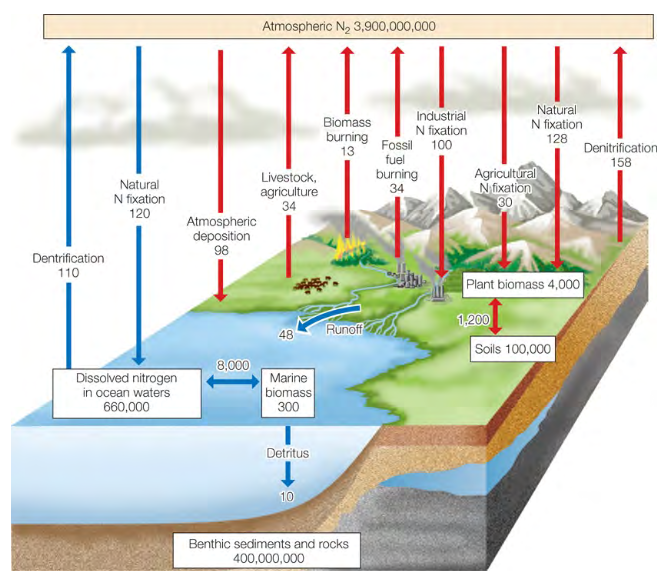
\includegraphics[width=5in]{global-nitrogen-cycle.png}
    \caption{The Global Nitrogen Cycle}
    \label{global-nitrogen}
\end{figure}

\paragraph{In Figure \ref{global-nitrogen}: The Global Nitrogen Cycle}
\begin{itemize}
    \item Largest
          \begin{itemize}
              \item Flux: Denitrification - gaseous loss of nitrogen from the soil converting into $N_2$ gas in the atmosphere.
              \item Pool: Atmospheric $N_2$
          \end{itemize}
    \item Anthropogenic fluxes
          \begin{itemize}
              \item Agricultural/Industrial Nitrogen fixation
              \item Fossil fuels, biomass burning, livestock
          \end{itemize}
\end{itemize}

\subsection{Linking Cycles}

\subsubsection{Runoff}

\begin{itemize}
    \item Runoff as a flux: being dissolved in water adds that compound to the water cycle, helping to move it around. All 3 cycles experience runoff.
    \item  Watersheds: Patterns of runoff across land.
\end{itemize}

\paragraph{The gulf of Mexico Dead Zone}
\begin{itemize}
    \item Cause
          \begin{itemize}
              \item Large portion of the Midwest is one watershed, runs off into the Gulf of Mexico.
              \item Chemical runoff: Municipal waste (poo), fertilizer (also poo)
              \item Nitrogen is often a limiting resource, so the nitrogen runoff from fertilizer and other poo causes an algal bloom.
              \item When the algae die, the decomposition of their bodies uses all of the oxygen in the water column.
              \item Low oxygen levels in water column along the coast of the Gulf of Mexico.
          \end{itemize}
    \item Reducing the Dead Zone
          \begin{itemize}
              \item Hurricanes/windstorms mix up water and infuse oxygen.
          \end{itemize}
    \item Impacts of Dead Zone
          \begin{itemize}
              \item Female fish in hypoxic locations have lower fecundity/smaller ovaries.
              \item Male fish have smaller testes and lower sperm production.
          \end{itemize}
\end{itemize}

\subsubsection{How the Carbon cycle connects to the Nitrogen Cycle}

\begin{itemize}
    \item Photosynthesis takes $CO_2$ out of the atmosphere and turns it into sugars.
    \item \textit{Rubisco} is the protein that actually picks up the $CO_2$ from the atmosphere.
    \item \textit{Rubisco} is made up of a lot of nitrogen.
    \item Plants require lots of nitrogen to capture $CO_2$.
\end{itemize}

% ========== ========== ========== ==========

\section{Energy and Trophics}

\subsection{Ecosystem Energy}

\subsection{Trophic Roles and Interactions}

% ========== ========== ========== ==========

\section{History of Life}

\subsection{Precambrian to Paleozoic}

\subsection{Mesozoic to Cenozoic}


\end{document}